\documentclass[10pt]{article}

%% --- Geometry / typography ---------------------------------------------------
\usepackage[margin=0.9in]{geometry}
\usepackage[T1]{fontenc}
\usepackage[utf8]{inputenc}
\usepackage{lmodern}
\usepackage{microtype}

%% --- Math / typography helpers ----------------------------------------------
\usepackage{amsmath,amssymb,amsthm}
\usepackage{bm}
\newtheorem{theorem}{Theorem}
\newtheorem{proposition}{Proposition}
\newtheorem{corollary}{Corollary}

%% --- Tables, figures, captions ----------------------------------------------
\usepackage{booktabs}
\usepackage{multirow}
\usepackage{tabularx}
\usepackage{array}
\usepackage{graphicx}
\graphicspath{{figures/}{../assets/paper1_figs/}{assets/paper1_figs/}}
\usepackage{float}
\usepackage{lscape}
% TinyTeX in this environment lacks pdflscape; add the PDF rotation attribute
% that makes lscape pages open upright in standard PDF viewers.
\makeatletter
\g@addto@macro\landscape{\clearpage\pdfpageattr{/Rotate 90}}
\g@addto@macro\endlandscape{\clearpage\pdfpageattr{}}
\makeatother
\usepackage[font=small,labelfont=bf,skip=4pt]{caption}
\usepackage{subcaption}

%% --- Code listing -----------------------------------------------------------
\usepackage{xcolor}
\usepackage{listings}
\lstset{
  basicstyle=\ttfamily\footnotesize,
  breaklines=true,
  columns=fullflexible,
  keywordstyle=\color{blue!60!black}\bfseries,
  commentstyle=\color{gray}\itshape,
  stringstyle=\color{purple!50!black},
  language=Python,
  showstringspaces=false,
  numberstyle=\footnotesize\color{gray},
  frame=single, framerule=0.3pt, framesep=4pt,
  backgroundcolor=\color{gray!4},
  xleftmargin=4pt,
  literate={σ}{{$\sigma$}}1 {ρ}{{$\rho$}}1 {ε}{{$\varepsilon$}}1
}

%% --- Hyperlinks / refs ------------------------------------------------------
\usepackage[hidelinks]{hyperref}
\usepackage{url}
\usepackage{cleveref}

%% --- Misc -------------------------------------------------------------------
\usepackage{enumitem}
\setlist{nosep,leftmargin=*}
\usepackage[normalem]{ulem}
% seqsplit lets long monospace identifiers (e.g. snake_case metric names) break
% across line ends, eliminating overfull \hbox warnings on long \code{...} runs.
\usepackage{seqsplit}
% Allow extra inter-word space on the last pass to absorb the occasional
% paragraph that microtype alone cannot fit; keeps the right margin tidy
% on lines that would otherwise overflow by a few points.
\emergencystretch=3em
\setlength{\textfloatsep}{9pt plus 2pt minus 2pt}
\setlength{\floatsep}{8pt plus 2pt minus 2pt}
\setlength{\intextsep}{8pt plus 2pt minus 2pt}
\makeatletter
\setlength{\@fptop}{0pt}
\setlength{\@fpsep}{8pt plus 2pt}
\setlength{\@fpbot}{0pt plus 1fil}
\makeatother

%% --- Macros -----------------------------------------------------------------
% Short code-style identifiers are used only for software names or compact protocol keys.
\newcommand{\code}[1]{\texttt{\small #1}}
\newcommand{\codebrk}[1]{\texttt{\small\seqsplit{#1}}}
\newcommand{\stdmax}{\ensuremath{\sigma_{\max}}}

\ifdefined\blindsubmission
  \newcommand{\paperauthors}{Anonymous Authors}
\else
  \newcommand{\arxivauthors}{Author names to be supplied for arXiv v1}
\newcommand{\paperpubliccodeurl}{https://github.com/Anguo-star/lewm-acpc-diagnostics}

  \newcommand{\paperauthors}{\arxivauthors}
\fi

\title{\textbf{Action-Conditioned Predictive Consistency\\as a Diagnostic for Gaussian-Noise Robustness\\in JEPA World Models}}
\author{\paperauthors}
\date{June 2026}
\hypersetup{
  pdftitle={Action-Conditioned Predictive Consistency as a Diagnostic for Gaussian-Noise Robustness in JEPA World Models},
  pdfkeywords={visual world models, JEPA, action-conditioned predictive consistency, visual robustness, predictive-dynamics diagnostics}
}

\begin{document}
\maketitle

\begin{abstract}
Latent predictive world models avoid pixel reconstruction, but pixel-free prediction is not a robustness definition for closed-loop control. We study this gap with action-conditioned predictive consistency (ACPC), a no-retraining diagnostic for JEPA-style control checkpoints. The compressed paper-facing diagnostic has two theory-aligned readouts: ACPC tail risk (ATR), the high-quantile same-state clean/noisy action-conditioned rollout disagreement, and selective-margin pass rate (SMPR), a task-grounded near-boundary check that action-relevant distinctions remain separated. Across three independent LeWM training seeds and four control tasks, no-noise checkpoints are fragile under observation-only Gaussian noise, while input-side noise training yields broad matched-Gaussian robustness plateaus. At recovered endpoints, ATR drops sharply and SMPR rises to near one across tasks. The claim is a controlled diagnostic for matched-Gaussian robustness plateaus, not a closed-loop stability guarantee, universal perturbation-transfer result, or new training objective.

\smallskip
\noindent\textbf{Keywords:} visual world models; JEPA; action-conditioned predictive consistency; visual robustness; predictive-dynamics diagnostics.
\end{abstract}

\smallskip
\ifdefined\blindsubmission
\noindent\textbf{Anonymous reproducibility note:} code and data availability follow the venue's double-blind supplemental policy.
\else
\noindent\textbf{Code and data release:} \url{\paperpubliccodeurl}
\fi

%% ===========================================================================
\section{Introduction}\label{sec:intro}

\subsection{Latent prediction is not a robustness definition}\label{sec:intro-heuristic}

JEPAs predict future representations instead of reconstructing pixels, which can reduce pressure to encode high-magnitude irrelevant visual detail~\cite{assran2023ijepa,bardes2024vjepa,vanassel2025jointembeddingreconstruction}. For control, however, ``irrelevant'' is action- and transition-dependent. A representation may ignore a background texture but must preserve a contact pose or doorway state if that changes the next useful action. Thus encoder-level invariance is an incomplete target: planning uses the model's \emph{predictions}, so robustness must be stated after action-conditioned prediction.

We use this failure as a controlled diagnostic probe. Across three independent LeWM~\cite{maes2026lewm} training seeds, the no-noise baseline remains strong on clean observations but loses $74.56 \pm 5.55$ points on PushT and $41.00 \pm 1.44$ points on Reacher under observation-only Gaussian noise at std $0.08$ with the goal unperturbed. Observation+goal noise is reported as a harder auxiliary stress condition. Test-time visual fragility is not new~\cite{kostrikov2020drq,yarats2022drqv2,hansen2021soda,vigmo}; our focus is what it reveals about JEPA latent world-model control.

\subsection{Operationalizing action-conditioned predictive consistency}\label{sec:intro-acpc}

We operationalize a downstream-control view of visual robustness for JEPA world models through \emph{action-conditioned predictive dynamics}. Let $z = E(h)$ and $\tilde z = E(\tilde h)$ be the latents an encoder $E$ produces from an unperturbed history $h$ and a perturbed history $\tilde h$ of the same underlying state, and let $F^{k}(\cdot,\mathbf a_{t:t+k-1})$ be the action-conditioned latent predictor rolled out for $k$ steps under an action sequence $\mathbf a$. We \emph{allow} $z \neq \tilde z$. The robustness target is placed \emph{after} the predictor: in task-relevant coordinates,
\begin{equation}
  F^{k}\!\big(z,\mathbf a_{t:t+k-1}\big) \;\approx\; F^{k}\!\big(\tilde z,\mathbf a_{t:t+k-1}\big), \qquad k = 1,\dots,H,
  \label{eq:intro-acpc}
\end{equation}
so that the two branches induce the same next-state and rollout predictions under the same action intervention. The requirement is \emph{selective}: it should hold only for nuisance perturbations of the same underlying state. State differences that change action-conditioned transitions, costs, or the optimal action must remain \emph{discriminable}, or the planner loses the distinctions it needs. We make both halves precise in \Cref{sec:acpc}.

This diagnostic view changes what counts as a useful robustness measurement. Encoder geometry is a useful first-stage diagnostic because it shows whether visual perturbations enter and reshape the latent neighborhood, but encoder-level latent closeness, $\lVert z-\tilde z\rVert \to 0$, is not a complete control-robustness definition: large nuisance shifts can wash out after prediction, whereas small shifts can still be amplified downstream. Planning, cost, and action metrics remain useful as \emph{downstream readouts} of predictive consistency; future objectives should regularize action-conditioned predictive dynamics while preserving action-relevant discriminability.

\subsection{Existing noisy-evaluation results as a controlled probe}\label{sec:intro-tension}

We use input-side noise augmentation as the controlled intervention. The \stdmax{} $\in \{0.01,\dots,0.08\}$ sweep across four tasks creates paired baseline/recovered checkpoints for asking whether closed-loop Gaussian recovery is accompanied by lower same-state predictive tail risk and preserved task-grounded separations. Because the sweep forms broad task-dependent plateaus under finite evaluation variance, we do not treat a single point-best \stdmax{} or small within-plateau score differences as meaningful checkpoint ordering. Appendix~\ref{sec:appendix-target-view} records a negative target-view ablation: perturbed-history $\to$ original-future denoising is not a sufficient closed-loop fix, so the retained empirical branch is full-sequence perturbed-target training.

\subsection{Contributions}\label{sec:intro-contributions}

\paragraph{C1 --- Selective ACPC principle.} Robustness diagnostics should require both low same-state action-conditioned predictive-disagreement tails and preserved task-grounded near-boundary separations. Low consistency loss alone is not enough, because collapse can also make noisy and clean views agree.

\paragraph{C2 --- Theory-matched compression.} ATR estimates the ACPC-tail term exposed by the sampled-pool analysis and local Gaussian sensitivity calculation. SMPR estimates the discriminability/no-collapse countercondition that makes low ATR meaningful. The clean-margin term remains a formal caveat explaining why the diagnostic is not a closed-loop guarantee.

\paragraph{C3 --- Fixed-checkpoint evidence.} Across three LeWM training seeds, matched-Gaussian robustness plateaus coincide with large ATR reductions and near-one SMPR at recovered endpoints. Unseen-stressor scores and negative ablations bound the scope without turning the diagnostic into a method or universal transfer claim.

%% ===========================================================================
\section{Related Work}\label{sec:related}

\subsection{Latent prediction and JEPA world models}
JEPA~\cite{lecun2022path} predicts in latent space rather than reconstructing pixels; I-JEPA~\cite{assran2023ijepa} and the V-JEPA family~\cite{bardes2024vjepa,assran2025vjepa2,murlabadia2026vjepa21} extend this idea to images, video, and dense physical-world representations. LeWM~\cite{maes2026lewm}, our baseline, stabilizes an end-to-end JEPA world model with SIGReg~\cite{eppspulley1983}. PLDM~\cite{sobal2022jointembeddingpredictivearchitectures,sobal2025stresstesting}, via \code{stable-worldmodel}~\cite{maes2026stableworldmodel}, provides related latent-dynamics planning context. LeJEPA theory~\cite{klindt2026lejepaworldmodel} studies latent-variable recovery and latent planning; our diagnostic asks whether learned visual world-model checkpoints give paired clean/noised views consistent action-conditioned predictions.

\subsection{Invariance, augmentation, and visual robustness}
Augmentation and joint-embedding losses impose invariances only when their training signal identifies the right nuisance factors~\cite{wang2020alignuniform,tamkin2023featuredropout,zhang2022rethinkaug}. Recent theory clarifies why latent prediction can help with nuisance or noisy features but also why it is not enough for control. Van Assel et al.~\cite{vanassel2025jointembeddingreconstruction} and Littwin et al.~\cite{littwin2024jepaavoidsnoisyfeatures} analyze representation-level effects; they do not address closed-loop action-conditioned rollout, candidate-cost stability, or the need to keep action-distinct states separable. Seq-JEPA~\cite{ghaemi2025seqjepa} addresses a related invariance--equivariance tension architecturally.

We do not train robust visual-control systems as competing baselines. DrQ/DrQ-v2~\cite{kostrikov2020drq,yarats2022drqv2}, SODA/DMC-GB~\cite{hansen2021soda}, DreamerV3~\cite{hafner2025dreamerv3}, TD-MPC2~\cite{hansen2024tdmpc2}, and ViGMO~\cite{vigmo} define future method-comparison axes; noisy/video JEPA variants~\cite{njepa2025,huang2026vjepa,usjepa2025} are representation-level context. ACPC is complementary: it tests whether same-state visual perturbations become equivalent after a fixed action intervention while action-, transition-, or cost-distinct cases remain discriminable.

\subsection{Control-relevant predictive representations}
Bisimulation merges states with equivalent reward and transition behavior. DeepMDP~\cite{gelada2019deepmdp}, DBC~\cite{zhang2021dbc}, bisimulation-regularized MPC~\cite{bsmpc}, and Bisim-JEPA~\cite{toso2026bisimjepa} use this principle to learn control-relevant representations. Value-equivalent and value-aware models~\cite{grimm2020valueequivalence,voelcker2025calibratedvalueaware} and VIBR~\cite{dupuis2023vibr} likewise emphasize downstream control consequences. Wang et al.~\cite{wang2026groupactions} formalize action-conditioned video world modeling as a group action with identity, inverse, and composition-consistency metrics. ReOI~\cite{chen2025reoi} treats visual distractor robustness in visual MPC through observation interventions for world-model action-outcome prediction. These lines show that downstream predictive consequences are already central to control-representation work. Our diagnostic instantiates that view for paired clean/noised JEPA latent-world-model rollouts: same-state noised and unperturbed views should agree after the same action sequence, while action-distinct transitions remain separable.

Our use of ACPC is therefore narrower than an identifiability theorem, a learned bisimulation metric, or a robust MPC intervention. LeJEPA-style results motivate latent prediction and planning under latent recovery assumptions; bisimulation and value-aware models define task abstractions; group-action metrics test action faithfulness; ReOI modifies observation handling for robust visual MPC. This paper instead supplies a JEPA checkpoint diagnostic centered on additive Gaussian pixel-noise stress tests: predictive stability is tested on paired same-state clean/noised rollouts under the same action sequence, fixed-candidate cost stability is derived as a sufficient condition, and a separate discriminability guard checks that action-, transition-, or cost-distinct cases have not been collapsed.

%% ===========================================================================
\section{Action-Conditioned Predictive Consistency}\label{sec:acpc}

This section defines action-conditioned predictive consistency and its discriminability countercondition. We use ACPC to separate two requirements that encoder invariance alone conflates: same-state visual perturbations should agree after action-conditioned rollout, while task-grounded different-state pairs should remain separable. \Cref{sec:acpc-diag} then maps these two requirements to ATR and SMPR.

\subsection{Setup and definitions}\label{sec:acpc-def}

Let $o_t$ be an unperturbed observation and $\tilde o_t = \tau(o_t)$ a visually perturbed view of the \emph{same} underlying state ($\tau$ is additive Gaussian pixel noise here, but the definitions are perturbation-agnostic). Let $h_t$ and $\tilde h_t$ be the corresponding observation--action histories, $E_\theta$ the encoder, and $F_\theta$ the action-conditioned latent predictor. Fix an action sequence $\mathbf a^H_t = a_{t:t+H-1}$ that is \emph{identical} on both branches. For compact notation below, $\mathbf a_{0:k-1}$ denotes the length-$k$ prefix of this sequence after re-indexing time at $t$, and we write
\begin{equation}
  z_t = E_\theta(h_t), \quad \tilde z_t = E_\theta(\tilde h_t), \qquad
  \hat z_{t+k} = F_\theta^{k}(z_t, \mathbf a_{0:k-1}), \quad
  \hat{\tilde z}_{t+k} = F_\theta^{k}(\tilde z_t, \mathbf a_{0:k-1}).
  \label{eq:acpc-objects}
\end{equation}
Let $\Pi$ denote a \emph{task-relevant predictive readout} --- the full latent, a transition delta, goal-distance or cost features, or a learned projection --- and let $d$ be a distance on its range.

\paragraph{Action-conditioned predictive consistency.} For a same-state perturbation pair under the shared action sequence,
\begin{equation}
  \mathrm{ACPC}_H(o_t, \tilde o_t, \mathbf a)
  = \sum_{k=1}^{H} \alpha_k \, d\!\big(\Pi(\hat z_{t+k}),\, \Pi(\hat{\tilde z}_{t+k})\big),
  \qquad \alpha_k \ge 0 .
  \label{eq:acpc-h}
\end{equation}
For the theoretical statements below, we use the induced horizon metric
\begin{equation}
  d_H\big((u_1,\ldots,u_H),(v_1,\ldots,v_H)\big)
  = \sum_{k=1}^{H}\alpha_k d(u_k,v_k),
  \label{eq:acpc-horizon-metric}
\end{equation}
so that \Cref{eq:acpc-h} is exactly the clean/perturbed rollout-readout distance under the shared action sequence. In experiments, ATR uses the 90th percentile of this normalized same-state rollout disagreement.
In this diagnostic framing, robustness corresponds to small $\mathrm{ACPC}_H$ together with action-relevant discriminability, not to the encoder distance $d(z_t, \tilde z_t)$ alone. Encoder closeness is a useful first-stage risk signal, but it is neither necessary (a large but task-irrelevant encoder shift can wash out through $F_\theta$ and $\Pi$) nor sufficient (a small encoder shift can still change the predicted future enough to flip the planned action).

\paragraph{Action-relevant discriminability (countercondition).} Consistency must be \emph{selective}. Let $Y^{H}(s,\mathbf a)$ denote a task-relevant future readout that is external to the learned predictor --- simulator state, cost-to-go, inverse-dynamics label, contact/keyframe tag, or another diagnostic proxy available in the dataset. For two genuinely different states $s_i, s_j$ (with latents $z_i, z_j$) that admit an action sequence under which this external future readout diverges,
\begin{equation}
  \Delta^{H}_{\mathrm{dyn}}(s_i, s_j, \mathbf a)
  = d_Y\!\big(Y^{H}(s_i, \mathbf a),\, Y^{H}(s_j, \mathbf a)\big) > m,
  \label{eq:acpc-disc-dyn}
\end{equation}
the representation and predictions should keep them separable,
\begin{equation}
  d\!\big(\Psi(z_i),\, \Psi(z_j)\big) > m',
  \label{eq:acpc-disc}
\end{equation}
where $\Psi$ is a discriminability readout, possibly action-conditioned (latent, predicted delta under $\mathbf a$, inverse-dynamics feature, cost feature, or rollout embedding), and $m, m' > 0$ are margins. Equations~\eqref{eq:acpc-h}--\eqref{eq:acpc-disc} state the target: lower predictive disagreement for same-state visual perturbations must preserve discriminability among state/action/transition-distinct pairs. A method that drove $\mathrm{ACPC}_H \to 0$ by collapsing the latent would violate \eqref{eq:acpc-disc}, so the two conditions are inseparable.

\subsection{Operational consistency diagnostics}\label{sec:acpc-diag}

The paper-facing diagnostic uses two readouts. ACPC Tail Risk (ATR) is the 90th percentile of normalized same-state clean/noisy ACPC-H rollout disagreement under a fixed recorded action sequence; lower is better. Selective Margin Pass Rate (SMPR) is the pass rate of task-grounded label-crossing pairs whose clean different-state rollout distance exceeds the same-state noisy radius at margin zero; higher is better. ATR measures predictive-stability tail risk, while SMPR rules out the collapse failure in which all states become indistinguishable. Encoder geometry and planner-side readouts are not separate paper-facing diagnostics in this compressed version.

\begin{table}[H]
\centering
\caption{Theory-to-metric mapping for compressed selective ACPC.}
\label{tab:theory-metric-map}
\small
\begin{tabularx}{\textwidth}{l l X}
\toprule
Core theorem quantity & Paper-facing readout & Role \\
\midrule
$\Pr[D>\epsilon]$ / ACPC tail & ATR & same-state action-conditioned predictive-stability tail \\
$d_{\mathrm{diff}}>d_{\mathrm{same}}+m$ & SMPR & task-grounded anti-collapse margin \\
\bottomrule
\end{tabularx}
\end{table}

\subsection{ACPC as a fixed-candidate stability condition}\label{sec:acpc-planner-stability}

ACPC is connected to planning through the candidate costs evaluated by model-predictive control. Let $h$ be a clean history, $\tilde h$ the corresponding perturbed history, and let both branches evaluate the same candidate action sequence $\mathbf a$. For a goal or task descriptor $g$, define
\begin{equation}
  C_h(\mathbf a, g)
  = J\!\left(\Pi(\hat z_{t+1}), \ldots, \Pi(\hat z_{t+H}), g\right),
  \label{eq:candidate-cost}
\end{equation}
where $J$ is the planner's cost readout on the rollout-readout sequence. $C_{\tilde h}(\mathbf a,g)$ is defined analogously from the perturbed branch. The following statements are sufficient conditions for stability on a fixed candidate set; they do not prove stability of the full CEM sampling distribution or of the closed-loop trajectory over repeated replanning.

\begin{proposition}[Encoder shift as one route to rollout disagreement]\label{prop:encoder-route}
Fix an action sequence $\mathbf a$ and write
\[
  G_{\mathbf a}(z)=\Pi(F_\theta^{1:H}(z,\mathbf a))
\]
for the rollout-readout map. If $G_{\mathbf a}$ is locally $L_G$-Lipschitz between $E_\theta(h)$ and $E_\theta(\tilde h)$ under encoder metric $d_Z$ and rollout-readout metric $d_H$, then
\[
 d_H\!\left(G_{\mathbf a}(E_\theta(h)),G_{\mathbf a}(E_\theta(\tilde h))\right)
 \le L_G\, d_Z\!\left(E_\theta(h),E_\theta(\tilde h)\right).
\]
\end{proposition}

\begin{proof}
This is the local Lipschitz condition applied to the two encoded histories.
\end{proof}

This bound makes encoder geometry a first-stage risk signal: small encoder shifts imply small rollout disagreement only under local insensitivity, large shifts can be contracted by $G_{\mathbf a}$, and small shifts can be amplified by the predictor or cost readout. This is why the empirical diagnostic measures the tail of action-conditioned rollout disagreement rather than encoder distance alone.

\begin{proposition}[ACPC controls candidate-cost drift]\label{prop:cost-drift}
Assume that $J$ is locally $L_J$-Lipschitz on the clean/perturbed rollout-readout neighborhood evaluated by the fixed candidate set under metric $d_H$. If
\[
 d_H\!\left(\Pi(F_\theta^{1:H}(E_\theta(h),\mathbf a)),
             \Pi(F_\theta^{1:H}(E_\theta(\tilde h),\mathbf a))\right) \le \epsilon,
\]
then
\[
 |C_h(\mathbf a,g)-C_{\tilde h}(\mathbf a,g)| \le L_J\epsilon .
\]
\end{proposition}

\begin{proof}
The inequality is the local Lipschitz condition applied directly to the clean and perturbed rollout-readout sequences.
\end{proof}

In the compressed diagnostic, this condition is instantiated by the L2 rollout-token distance whose high-quantile tail defines ATR; empirical companion audits are kept outside the paper-facing metric set.

\begin{proposition}[Candidate top-1 stability]\label{prop:top1-stability}
Let $\mathcal A=\{\mathbf a^1,\ldots,\mathbf a^K\}$ be the shared candidate set. Assume lower cost is preferred, and let $\mathbf a^{(1)}$ and $\mathbf a^{(2)}$ denote the lowest- and second-lowest-cost candidates on the clean branch. Suppose that for every candidate $j$,
\[
 |C_h(\mathbf a^j,g)-C_{\tilde h}(\mathbf a^j,g)|\le \eta .
\]
If the clean branch has a strict top-1/top-2 margin
\[
\Delta = C_h(\mathbf a^{(2)},g)-C_h(\mathbf a^{(1)},g) > 2\eta,
\]
then the perturbed branch selects the same top-1 candidate.
\end{proposition}

\begin{proof}
For any candidate $\mathbf a^j \neq \mathbf a^{(1)}$,
\[
C_{\tilde h}(\mathbf a^j,g)-C_{\tilde h}(\mathbf a^{(1)},g)
\ge
C_h(\mathbf a^j,g)-C_h(\mathbf a^{(1)},g)-2\eta
\ge \Delta-2\eta >0 .
\]
Thus every non-top candidate remains more costly than the clean top-1 candidate on the perturbed branch.
\end{proof}

\begin{corollary}[ACPC-margin condition for candidate stability]\label{cor:acpc-margin}
Let $\mathcal A=\{\mathbf a^1,\ldots,\mathbf a^K\}$ be a shared candidate set and assume the cost readout $J$ is locally $L_J$-Lipschitz as in Proposition~\ref{prop:cost-drift}. If every candidate in $\mathcal A$ has rollout-readout discrepancy at most $\epsilon$ between the clean and perturbed branches, and the clean branch has top-1/top-2 margin $\Delta > 2L_J\epsilon$, then the two branches select the same top-1 candidate from $\mathcal A$.
\end{corollary}

\begin{proof}
Proposition~\ref{prop:cost-drift} gives $|C_h(\mathbf a^j,g)-C_{\tilde h}(\mathbf a^j,g)|\le L_J\epsilon$ for every candidate. Applying Proposition~\ref{prop:top1-stability} with $\eta=L_J\epsilon$ gives the result.
\end{proof}

The corollary gives a formal link between ACPC and fixed-candidate decisions without turning the diagnostic into a closed-loop guarantee. It connects paired predictive agreement to candidate-cost stability and then to action selection under a margin condition. The result is limited to a fixed candidate set; adaptive sampling, repeated replanning, and environment feedback can still change the closed-loop trajectory.


\subsection{Sampled-pool stability and Gaussian sensitivity}\label{sec:acpc-sampled-gaussian}

The fixed-candidate statement is the deterministic core. A sampled candidate pool adds finite-sample risk. The next bound keeps the same diagnostic scope while exposing why ATR must be a tail readout and why clean candidate margins remain a caveat.

\begin{theorem}[Sampled-pool ACPC stability]\label{thm:sampled-pool-acpc}
Let $\mathcal A=\{\mathbf a^1,\ldots,\mathbf a^K\}\sim q^K$ be a once-sampled candidate pool, and use deterministic tie-breaking for $\arg\min$. For each sampled candidate define
\[
D_j = d_H\!\left(\Pi(F_\theta^{1:H}(E_\theta(h),\mathbf a^j)),
                  \Pi(F_\theta^{1:H}(E_\theta(\tilde h),\mathbf a^j))\right).
\]
Assume $J$ is locally $L_J$-Lipschitz on the evaluated rollout-readout neighborhood and that a single draw from $q$ satisfies
\[
\Pr_{\mathbf a\sim q}[D(\mathbf a)>\epsilon]\le \delta .
\]
Let $\Delta_{\mathcal A}=C_h(\mathbf a^{(2)},g)-C_h(\mathbf a^{(1)},g)$ be the clean branch top-1/top-2 margin inside the sampled pool. Then
\[
\Pr_{\mathcal A}\!\left[
\arg\min_j C_h(\mathbf a^j,g) \ne
\arg\min_j C_{\tilde h}(\mathbf a^j,g)
\right]
\le
K\delta + \Pr_{\mathcal A}[\Delta_{\mathcal A}\le 2L_J\epsilon].
\]
\end{theorem}

\Cref{thm:sampled-pool-acpc} is not a convergence theorem for adaptive planning. It controls the instability of one sampled candidate pool. The first term is the probability that at least one candidate has a large clean/noisy rollout discrepancy, which motivates ATR. The second term is the probability that the clean candidate pool has too small a top-1 margin; it explains why ATR is not a closed-loop guarantee. SMPR is separate from this flip bound: it is the selective-discriminability condition required to make low ATR meaningful rather than collapsed.

\begin{corollary}[Replanning union bound]\label{cor:replanning-union}
If replanning step $t$ has sampled-pool flip-probability bound
\[
r_t=K_t\delta_t+\Pr[\Delta_{\mathcal A_t}\le 2L_J\epsilon_t],
\]
then over $T$ replanning steps,
\[
\Pr[\exists t\le T:\ \text{the sampled-pool top-1 flips at step }t]
\le \sum_{t=1}^{T} r_t .
\]
\end{corollary}

\begin{proposition}[Finite-sample tail calibration for paired diagnostics]\label{prop:finite-sample-tail-calibration}
Fix the diagnostic sampling distribution used to draw independent paired clean/noisy histories and candidate action sequences. Let
\[
X_i=\mathbf 1[D_i>\epsilon], \qquad i=1,\ldots,n,
\]
where $D_i$ is the paired ACPC rollout-readout discrepancy for diagnostic item $i$. Let $p_\epsilon=\Pr[D>\epsilon]$ and $\hat p_\epsilon=n^{-1}\sum_i X_i$. Then, with probability at least $1-\delta$ over the diagnostic sample,
\[
p_\epsilon \le \hat p_\epsilon + \sqrt{\frac{\log(1/\delta)}{2n}}.
\]
The same one-sided calibration applies to SMPR after fixing its task-grounded pair construction.
\end{proposition}

This calibration is with respect to the fixed diagnostic sampling distribution and its independent-sample idealization. It does not convert an empirical quantile or pass-rate table into a uniform bound over all closed-loop states; when nearby dataset windows are dependent, we use it only as calibration.

The Gaussian stressor also has a local sensitivity interpretation. Let $G_{\mathbf a}(z)=\Pi(F_\theta^{1:H}(z,\mathbf a))$ and let $\tilde o=o+\xi$ with $\xi\sim\mathcal N(0,\sigma^2 I)$.

\begin{proposition}[Local Gaussian ACPC sensitivity]\label{prop:gaussian-sensitivity}
If $E_\theta$ and $G_{\mathbf a}$ are locally twice differentiable around $o$ and $E_\theta(o)$ with bounded second-order remainders, then for small $\sigma$,
\[
G_{\mathbf a}(E_\theta(o+\xi))-G_{\mathbf a}(E_\theta(o))
=
J_{G_{\mathbf a}}(E_\theta(o))J_E(o)\xi + R_\xi,
\]
where the remainder contributes higher-order terms, and
\[
\mathbb E_\xi\!\left[
\left\|G_{\mathbf a}(E_\theta(o+\xi))-G_{\mathbf a}(E_\theta(o))\right\|_2^2
\right]
=
\sigma^2\left\|J_{G_{\mathbf a}}(E_\theta(o))J_E(o)\right\|_F^2 + O(\sigma^3).
\]
\end{proposition}

Thus Gaussian ACPC measures action-conditioned encoder--predictor sensitivity, not encoder invariance alone. Small encoder shifts can still be amplified by $J_{G_{\mathbf a}}$, while large nuisance shifts can become harmless after rollout if the product $J_{G_{\mathbf a}}J_E$ is small in those directions. The selective target is therefore asymmetric: the product should be small along nuisance perturbation directions, while rollout readouts for action-relevant state differences remain separated. The task-grounded near-boundary proxy margin pass event used later is
\[
M=\mathbf 1\!\left[d_{\mathrm{proxy\ diff}}>d_{\mathrm{same\ state\ noise}}+\delta_m\right],
\]
with $\delta_m=0$ in the reported table. It is a finite state-proxy selective-consistency check, not a full semantic-label coverage guarantee.

The theoretical statements in this section are intended as diagnostic calibration rather than as closed-loop control guarantees. They identify the failure modes that a paired clean/noisy diagnostic should measure: rollout-disagreement tails, clean candidate-margin caveats, and collapse of task-grounded separations. They do not assert that a low empirical ATR is a uniform bound for adaptive planning, repeated replanning, or environment-feedback stability.

\paragraph{Selective ACPC pseudo-metric.}
For a nonempty fixed candidate family $\mathcal A$, the stability condition can be summarized by
\begin{equation}
  D_{\mathrm{ACPC}}^{\mathcal A}(h,\tilde h)
  =
  \max_{\mathbf a \in \mathcal A}
  d_H\!\left(\Pi(F_\theta^{1:H}(E_\theta(h),\mathbf a)),
             \Pi(F_\theta^{1:H}(E_\theta(\tilde h),\mathbf a))\right).
  \label{eq:acpc-pseudometric}
\end{equation}
When $d_H$ is a metric (or a pseudo-metric, if some horizon weights vanish), $D_{\mathrm{ACPC}}^{\mathcal A}$ is a pseudo-metric on histories after passing through the encoder, predictor, and readout: distinct histories can have zero distance if all candidate rollouts are readout-equivalent. This follows because each map $h\mapsto \Pi(F_\theta^{1:H}(E_\theta(h),\mathbf a))$ pulls back $d_H$ to a pseudo-metric, and the pointwise maximum of pseudo-metrics is again a pseudo-metric. The useful object is therefore \emph{selective} predictive stability. Small $D_{\mathrm{ACPC}}^{\mathcal A}$ for same-state visual perturbations gives candidate-cost and top-1 stability under the preceding Lipschitz and margin assumptions; the same contraction is not desirable for state/action pairs whose external task readouts differ, which is why the discriminability guard is part of the definition rather than an auxiliary aesthetic check.

\begin{corollary}[Fixed-candidate predictive stability]\label{cor:selective-stability}
Assume $D_{\mathrm{ACPC}}^{\mathcal A}(h,\tilde h)\le\epsilon$ for a same-state visual-perturbation pair and that $J$ is locally $L_J$-Lipschitz on the rollout readout. If the clean candidate margin satisfies $\Delta>2L_J\epsilon$, then the clean and perturbed branches select the same top-1 candidate from the fixed set $\mathcal A$.
\end{corollary}

\begin{proof}
By definition of $D_{\mathrm{ACPC}}^{\mathcal A}$, every candidate in $\mathcal A$ has rollout-readout discrepancy at most $\epsilon$. Proposition~\ref{prop:cost-drift} bounds the cost drift of every candidate by $L_J\epsilon$, and Proposition~\ref{prop:top1-stability} gives top-1 stability when $\Delta>2L_J\epsilon$.
\end{proof}

The statement becomes selective only when it is paired with a discriminability condition such as \Cref{eq:acpc-disc}. Without that second condition, fixed-candidate predictive stability can still be achieved by a collapsed encoder--predictor, as shown next.

Encoder closeness is not the right substitute for this condition. It is not necessary: a nuisance-subspace change can move $E_\theta(h)$ and $E_\theta(\tilde h)$ far apart while leaving $\Pi(F_\theta^{1:H}(\cdot,\mathbf a))$ and the cost unchanged. It is not sufficient either: a small encoder displacement can flip a low-margin cost ranking when the predictor or cost readout has high local sensitivity.

\begin{proposition}[ACPC alone permits collapse]\label{prop:acpc-collapse}
There exist encoder--predictor pairs for which $\mathrm{ACPC}_H=0$ for every same-state perturbation pair and every action sequence, while action-distinct states are mapped to identical rollout readouts.
\end{proposition}

\begin{proof}
Let $E_\theta(h)=z_0$ for every history and let $F_\theta^k(z_0,\mathbf a)=u_0$ for every horizon $k$ and action sequence $\mathbf a$. Then clean and perturbed branches always have identical rollout readouts, so same-state ACPC is zero. However, any two states that require different actions, costs, or transitions also have identical readouts, violating the discriminability condition in \Cref{eq:acpc-disc}.
\end{proof}

Thus low ACPC is meaningful only with a guard on action-relevant separation. This is the role of SMPR in the paper-facing diagnostic, and it is the failure exposed by the heteroscedastic-loss ablation in Appendix~\ref{sec:appendix-D}. This is where ACPC differs from existing nuisance-feature analyses of latent prediction: those results help explain why latent prediction may suppress irrelevant or noisy features at the representation level, whereas the condition above asks whether the remaining perturbation changes action-conditioned rollout readouts while preserving task-grounded separations.

%% ===========================================================================
\section{Study protocol}\label{sec:bg}

\subsection{Models and noise intervention}\label{sec:bg-models}

LeWM~\cite{maes2026lewm} is an end-to-end JEPA world model trained with a latent prediction loss and SIGReg regularization for latent-space model-predictive control. PushT (2D pushing), TwoRoom (2D navigation), Reacher (2D arm), and Cube (3D manipulation) form a heterogeneous stress panel spanning different nuisance/discriminability regimes. We add per-frame Gaussian noise to the input sequence as a full-sequence augmentation: each frame is independently noised with probability $p=1.0$, and the standard deviation is drawn from $\mathrm{Uniform}(0,\stdmax{})$. Because the target future frame is also encoded from the noised sequence, this intervention is not an original-target denoising objective. We sweep \stdmax{} $\in \{0.01,\dots,0.08\}$ and evaluate observation-only Gaussian noise with the goal image unperturbed as the primary robustness endpoint. Observation+goal Gaussian noise is retained as an auxiliary stress condition.

\subsection{Evaluation and diagnostics}\label{sec:bg-protocol}

The canonical LeWM development grid contains 36 epoch-10 checkpoints for training seed 3072: four tasks and, for each task, a no-noise baseline plus eight noise-trained checkpoints. Each checkpoint is evaluated with three evaluation seeds (42/43/44) and 100 trajectories per seed; canonical tables report the population mean $\pm$ population std across those three evaluation seeds. A completed Gaussian training-seed replication adds independent LeWM training seeds 3073 and 3074 under the same nine-point Gaussian sweep and evaluation protocol. Together, seed 3072 plus replication seeds 3073/3074 provide three training seeds for the main Gaussian closed-loop endpoint in \Cref{tab:training-seed-gaussian-lockbox}.

The main results follow the compressed evidence chain used in the claims. Closed-loop tables report training-seed mean/std for Gaussian robustness. ATR measures whether same-state clean/noisy rollout-disagreement tails contract at recovered endpoints, and SMPR checks whether task-grounded near-boundary separations survive that contraction. Unseen-stressor scores and negative ablations are auxiliary scope checks rather than additional core diagnostics.


%% ===========================================================================
\section{Experiments}\label{sec:exp}

The experiments use additive Gaussian pixel noise as the primary controlled stressor for a representation-diagnostic question. We first show that the stressor changes closed-loop behavior. We then ask where recovery appears in the model, prioritizing cross-task ACPC/paired-rollout evidence and keeping task-specific representation measurements only as discriminability checks. The study is a matched-stressor trace through the encoder--predictor--planner chain; point-best noise-level ranking, external method comparison, and broad perturbation-family transfer are outside its scope.

All results use the protocol in Section~\ref{sec:bg}: LeWM-base denotes the no-noise checkpoint, and LeWM+noise denotes the eight-level \stdmax{} sweep.

\subsection{JEPA control fragility under Gaussian observation noise}\label{sec:exp-cliff}

\Cref{tab:noise-cliff} reports LeWM-base success rates under unperturbed and noised evaluation. Each training-seed value is first averaged over the three evaluation seeds; the table reports mean $\pm$ population std across the three training seeds.

\begin{table}[H]
\centering
\caption{LeWM-base under test-time Gaussian-noise settings. Values are mean $\pm$ population std across three training seeds; each training-seed value averages three evaluation seeds $\times$ 100 trajectories. Drop is computed per training seed as clean success minus observation-noise 0.08 success, then summarized.}
\label{tab:noise-cliff}
\small
\setlength{\tabcolsep}{3pt}
\begin{tabular}{lrrrrr}
\toprule
Task & unpert. & obs 0.05 & obs 0.08 & obs+goal 0.08 & drop \\
\midrule
TwoRoom & $94.67 \pm 0.72$ & $81.33 \pm 6.77$ & $68.78 \pm 2.45$ & $53.56 \pm 2.57$ & $25.89 \pm 2.38$ \\
PushT   & $81.78 \pm 4.89$ & $19.22 \pm 9.12$ & $\phantom{0}7.22 \pm 5.81$ & $\phantom{0}4.89 \pm 1.64$ & $74.56 \pm 5.55$ \\
Reacher & $59.22 \pm 1.03$ & $33.56 \pm 1.77$ & $18.22 \pm 0.42$ & $13.78 \pm 1.50$ & $41.00 \pm 1.44$ \\
Cube    & $65.22 \pm 1.10$ & $46.67 \pm 1.96$ & $43.11 \pm 3.27$ & $45.78 \pm 0.79$ & $22.11 \pm 2.78$ \\
\bottomrule
\end{tabular}
\end{table}

LeWM-base is strong on unperturbed images, but observation noise alone already produces large closed-loop drops: PushT loses $74.56 \pm 5.55$ pts at observation-noise 0.08, Reacher $41.00 \pm 1.44$ pts, TwoRoom $25.89 \pm 2.38$ pts, and Cube $22.11 \pm 2.78$ pts. The observation+goal column shows the stronger full-input-stream Gaussian-noise stress case; it further degrades TwoRoom and Reacher, but is not the primary robustness endpoint because the goal image is also perturbed. The drop pattern across tasks remains informative: PushT degrades most sharply, consistent with contact-heavy continuous control being sensitive to visual precision.

\subsection{Noise augmentation supplies recovered checkpoints for diagnosis}\label{sec:exp-sweep}

\Cref{tab:sweep-summary} summarizes the sweep points needed for the main argument. All entries use the unified $n = 3$ evaluation seeds (42/43/44) $\times$ 100 trajectories protocol.

\begin{table}[H]
\centering
\caption{LeWM noise-sweep summary. Values are success rate mean $\pm$ population std across evaluation seeds. The two point-best columns may refer to different training-noise levels; they summarize the sweep envelope rather than a point-optimal checkpoint claim.}
\label{tab:sweep-summary}
\small
\setlength{\tabcolsep}{4pt}
\renewcommand{\arraystretch}{1.12}
\begin{tabularx}{\textwidth}{lrrrr>{\raggedright\arraybackslash}X}
\toprule
Task & unpert. base & obs 0.08 base & best clean row & best obs0.08 row & Main reading \\
\midrule
TwoRoom & $94.00 \pm 3.56$ & $65.67 \pm 1.25$ & $98.33 \pm 0.47$ (0.08) & $97.67 \pm 0.94$ (0.08) & large recovery; visually redundant regime \\
PushT & $86.33 \pm 2.36$ & $4.33 \pm 1.25$ & $89.67 \pm 1.70$ (0.03) & $89.00 \pm 4.32$ (0.08) & large recovery; contact-sensitive state \\
Reacher & $58.67 \pm 1.25$ & $18.33 \pm 2.05$ & $86.00 \pm 2.94$ (0.06) & $84.67 \pm 5.19$ (0.07) & recovery plus fixed-epoch clean lift \\
Cube & $66.67 \pm 2.62$ & $47.00 \pm 6.38$ & $69.33 \pm 0.47$ (0.01) & $68.33 \pm 2.49$ (0.03) & weaker recovery signal \\
\bottomrule
\end{tabularx}
\end{table}

\begin{figure}[H]
\centering
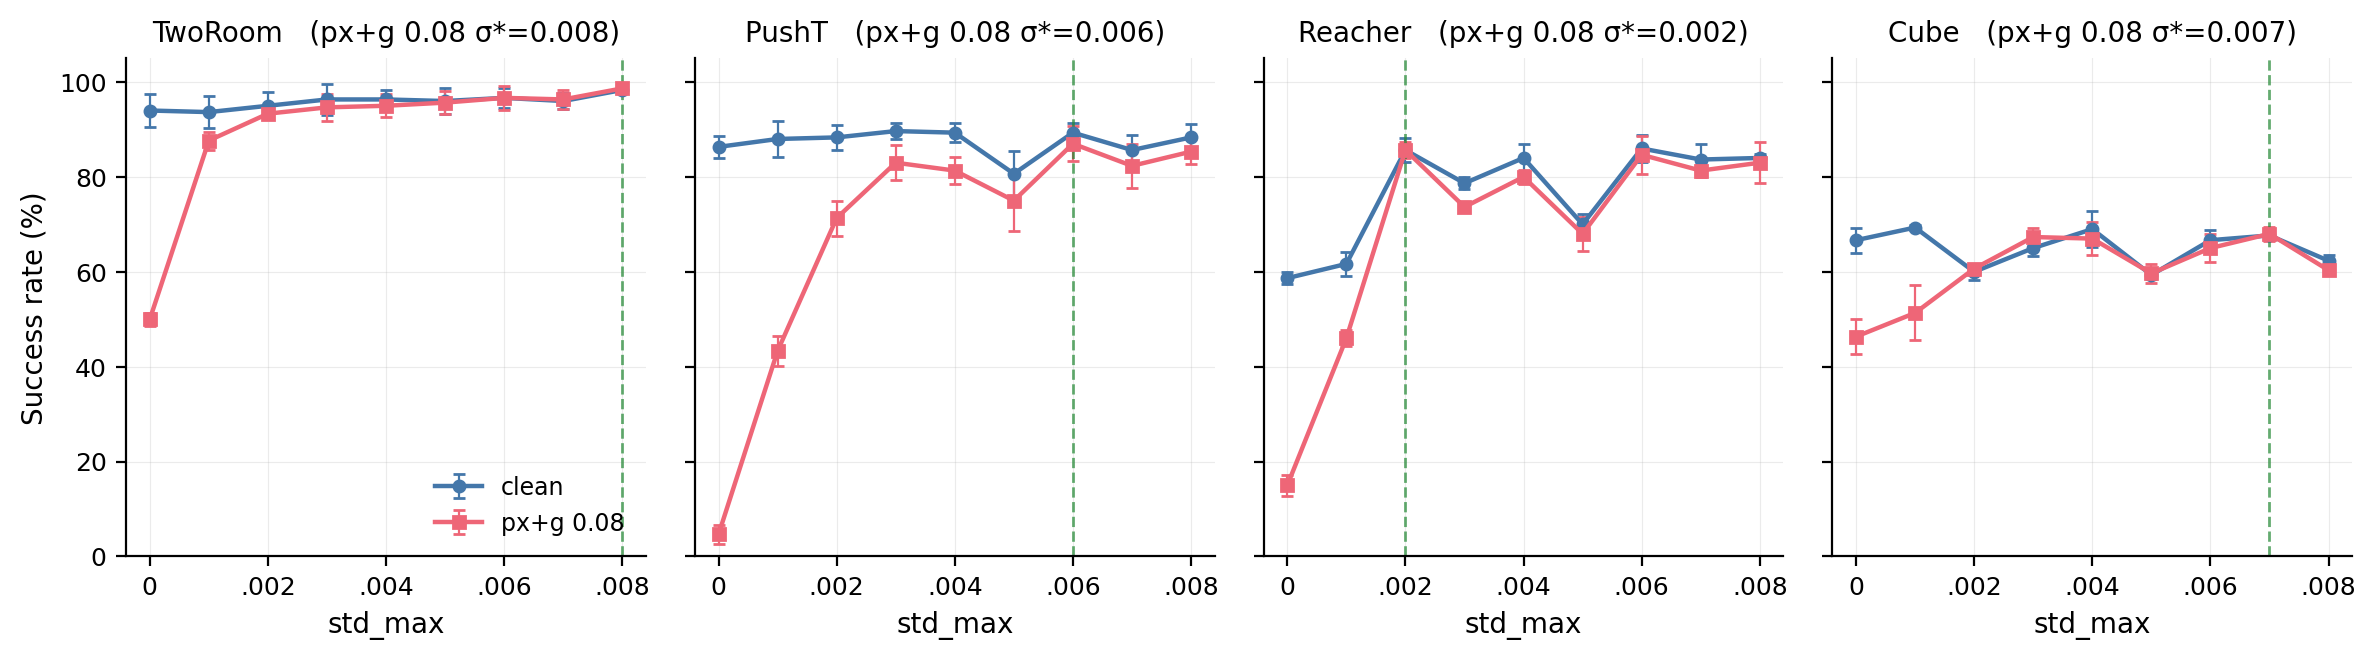
\includegraphics[width=\linewidth]{fig2_sweep.png}
\caption{Noise-training sweep across four tasks. Blue circles: unperturbed evaluation; red squares: observation-only Gaussian noise $\sigma=0.08$ with an unperturbed goal. Error bars show the population standard deviation across the three evaluation seeds. The curves document broad task-dependent recovery plateaus rather than point-optimal ranking.}
\label{fig:sweep}
\end{figure}

The sweep contributes two observations to the main argument. First, input-side noise can be an effective intervention in this protocol: PushT recovers from $4.33\%$ to $89.00\%$ at observation-noise 0.08, and Reacher from $18.33\%$ to $84.67\%$. Second, the grid supplies representative recovered checkpoints for the downstream diagnostic question: what changed in the encoder--predictor--planner chain?

Reacher also shows a fixed-epoch clean-control lift. Noise training improves not only observation-noise robustness but also unperturbed control: the representative clean row rises from $58.67\%$ at the no-noise baseline to about $86\%$ under noise training. We interpret this as a fixed-protocol regularization or stabilization effect rather than pure robustness recovery. The three-training-seed replication below makes the endpoint less dependent on seed 3072, but longer learning curves would still be needed to separate regularization from optimization timing.

The completed Gaussian training-seed replication strengthens the closed-loop part of the claim. It repeats the full Gaussian sweep for LeWM seeds 3073 and 3074 and combines them with the canonical seed-3072 sweep. \Cref{tab:training-seed-gaussian-lockbox} summarizes the observation-only Gaussian endpoint across all three training seeds.

\begin{table}[H]
\centering
\caption{Three-training-seed Gaussian replication for LeWM. Values are mean $\pm$ population std across training seeds 3072/3073/3074; each seed point is itself the mean over evaluation seeds 42/43/44 with 100 trajectories per eval seed. The endpoint is observation-only Gaussian evaluation at 0.08 with the goal image unperturbed. Regret is best obs 0.08 minus the fixed \stdmax{} $=0.08$ endpoint; the best-\stdmax{} range shows the task/seed-dependent plateau.}
\label{tab:training-seed-gaussian-lockbox}
\small
\setlength{\tabcolsep}{3pt}
\renewcommand{\arraystretch}{1.08}
\begin{tabularx}{\textwidth}{lccccc>{\raggedright\arraybackslash}X}
\toprule
Task & base obs 0.08 & std0.08 obs 0.08 & gain & best obs 0.08 & regret & best \stdmax{} range \\
\midrule
TwoRoom & $68.78 \pm 2.46$ & $97.11 \pm 0.57$ & $28.33 \pm 2.68$ & $97.67 \pm 0.27$ & $0.56 \pm 0.79$ & $0.05$--$0.08$ \\
PushT & $\phantom{0}7.22 \pm 5.81$ & $85.78 \pm 3.45$ & $78.56 \pm 5.18$ & $87.67 \pm 0.98$ & $1.89 \pm 2.67$ & $0.04$--$0.08$ \\
Reacher & $18.22 \pm 0.42$ & $81.55 \pm 0.88$ & $63.34 \pm 1.25$ & $83.78 \pm 0.63$ & $2.22 \pm 0.87$ & $0.05$--$0.07$ \\
Cube & $43.11 \pm 3.27$ & $62.56 \pm 1.55$ & $19.45 \pm 4.53$ & $66.44 \pm 1.34$ & $3.89 \pm 2.20$ & $0.03$--$0.05$ \\
\bottomrule
\end{tabularx}
\end{table}

Across three training seeds, the no-noise checkpoints retain large observation-noise cliffs, while the \stdmax{} $=0.08$ endpoint is within 0.56--3.89 pp of each task's best obs0.08 row. PushT remains the sharpest stress case, improving by $78.56 \pm 5.18$ points at the fixed high-noise endpoint; Reacher improves by $63.34 \pm 1.25$ points. The nonzero regret and task-dependent best-\stdmax{} ranges support plateau wording rather than a universal optimum at exactly \stdmax{} $=0.08$.

A three-seed blur/resize score check is reported in Appendix~\ref{sec:appendix-unseen-transfer}. It is an auxiliary severe-stressor check, not part of the matched-Gaussian claim. The next subsection asks whether the recovered Gaussian endpoints also move in the two compressed diagnostic readouts.

\subsection{Compressed selective-ACPC diagnostics}\label{sec:exp-compressed-diagnostics}

For the paper-facing diagnostic, ATR is the 90th percentile of same-state clean/noisy ACPC-H rollout distance normalized by the clean transition scale. SMPR is the task-grounded near-boundary selective-margin pass rate at margin zero. Both are computed without retraining on the fixed no-noise and \stdmax{} $=0.08$ checkpoints for training seeds 3072/3073/3074. \Cref{tab:compressed-selective-acpc} reports population mean/std across training seeds.

\begin{table}[H]
\centering
\caption{Compressed selective-ACPC diagnostics over training seeds 3072/3073/3074. ATR is the q90 normalized same-state clean/noisy action-conditioned rollout disagreement; lower is better. SMPR is the task-grounded near-boundary selective-margin pass rate; higher is better.}
\label{tab:compressed-selective-acpc}
\small
\setlength{\tabcolsep}{4pt}
\begin{tabular}{lrrrr}
\toprule
Task & ATR base & ATR std0.08 & SMPR base & SMPR std0.08 \\
\midrule
TwoRoom & $1.509 \pm 0.010$ & $0.111 \pm 0.016$ & $0.34 \pm 0.05$ & $0.99 \pm 0.01$ \\
PushT & $3.580 \pm 0.260$ & $0.247 \pm 0.017$ & $0.44 \pm 0.17$ & $1.00 \pm 0.00$ \\
Reacher & $2.628 \pm 0.048$ & $0.082 \pm 0.005$ & $0.73 \pm 0.03$ & $1.00 \pm 0.00$ \\
Cube & $2.320 \pm 0.045$ & $0.100 \pm 0.007$ & $0.45 \pm 0.03$ & $1.00 \pm 0.00$ \\
\bottomrule
\end{tabular}
\end{table}

The two readouts move in the intended selective direction on all four tasks: recovered endpoints have much smaller same-state predictive tails and much higher task-grounded margin pass rates. This does not make ATR/SMPR a point-ranking rule inside a plateau. Cube remains the useful boundary case: the compressed diagnostics improve strongly, but the closed-loop Gaussian gain and regret in \Cref{tab:training-seed-gaussian-lockbox} are weaker than PushT or Reacher, so closed-loop evaluation remains the behavioral authority.

SMPR uses programmatic task-state proxy labels, not oracle semantic annotations: TwoRoom uses doorway/room-side labels, PushT uses T-block pose cells, Reacher uses target/end-effector relation bins, and Cube uses cube-pose/goal-relation cells. Each anchor selects the closest label-crossing neighbor inside the closest 35\% state-distance neighborhood and passes if that clean different-state rollout distance exceeds the same-state noisy radius. The no-noise baselines are weak under this stricter audit, while the high-noise endpoint reaches near-one pass rate; stronger hand-labeled or simulator-derived contact, topology, action-value, or cost-to-go labels remain future validation.

\subsection{Bounded unseen-stressor check}\label{sec:exp-unseen-scope}

The main claim remains matched Gaussian-noise robustness. After freezing the Gaussian grid, we ran strongest-severity unseen-stressor score checks to test whether the fixed \stdmax{} $=0.08$ endpoint transfers outside the training perturbation family. \Cref{tab:unseen-scope-main} reports behavior only. TwoRoom and Reacher improve under strongest blur, whereas PushT and Cube do not show a clear resize gain at the scale of training-seed and evaluation variance. We use this as bounded behavior outside the matched Gaussian setting, not as a universal cross-perturbation robustness claim.

\begin{table}[H]
\centering
\caption{Bounded unseen-stressor score check. Values are mean $\pm$ population std across LeWM training seeds 3072/3073/3074; each seed point averages evaluation seeds 42/43/44 from strongest-severity unseen runs. Stress $\Delta$ is the fixed $\stdmax{}=0.08$ checkpoint minus the no-noise baseline.}
\label{tab:unseen-scope-main}
\small
\setlength{\tabcolsep}{4pt}
\begin{tabularx}{\textwidth}{llrrr>{\raggedright\arraybackslash}X}
\toprule
Task & stress & baseline stress & std0.08 stress & stress $\Delta$ & reading \\
\midrule
TwoRoom & blur $k=15$ & $47.67 \pm 5.44$ & $90.78 \pm 5.38$ & $+43.11 \pm 8.90$ & clear score gain \\
Reacher & blur $k=15$ & $22.00 \pm 3.78$ & $71.22 \pm 1.10$ & $+49.22 \pm 3.29$ & clear score gain \\
PushT & resize $0.25$ & $63.44 \pm 14.05$ & $66.33 \pm 8.38$ & $+2.89 \pm 17.98$ & no clear gain \\
Cube & resize $0.25$ & $57.00 \pm 1.96$ & $56.11 \pm 0.57$ & $-0.89 \pm 1.40$ & no clear gain \\
\bottomrule
\end{tabularx}
\end{table}

%% ===========================================================================
\section{Discussion and limitations}\label{sec:disc}

\paragraph{What the evidence supports.}
This is a controlled diagnostic study, not a method paper. Closed-loop evaluation establishes the behavior; ATR checks whether same-state noisy views have small action-conditioned predictive tails; SMPR checks whether task-grounded near-boundary distinctions survive that contraction. The primary statistic is the full three-training-seed Gaussian replication, with evaluation-seed variance kept as the within-seed measurement scale. These standard deviations are descriptive over three training seeds, not asymptotic significance claims.

\paragraph{Scope.}
Gaussian pixel noise remains the training/evaluation axis. The blur/resize rows are bounded behavior outside the matched Gaussian setting, not a transfer theorem. ATR/SMPR are not a point-best \stdmax{} predictor and do not replace closed-loop evaluation inside a broad plateau. We do not claim superiority over DrQ-style augmentation, TD-MPC2, DreamerV3, or robust MPC methods; the contribution is a no-retraining diagnostic for JEPA latent world-model checkpoints under a controlled Gaussian stressor.

\paragraph{What remains.}
The results argue against a too-strong reading of latent prediction: future-latent prediction alone does not guarantee closed-loop visual robustness. Stronger discriminability evidence would require hand-labeled or simulator-derived contact, topology, action-value, or cost-to-go labels, especially for PushT and Cube. The heteroscedastic NLL probe and target-view ablation bound the method story: prediction difficulty alone is the wrong gate, and perturbed-history $\to$ original-future targets are not sufficient here. Future methods can turn ATR/SMPR into objectives, but this paper keeps that as a separate method-paper path after diagnostic validity is established.

%% ===========================================================================
\section{Conclusion}\label{sec:conc}

This paper frames Gaussian-noise robustness in JEPA latent world-model control as a selective diagnostic problem. Closed-loop behavior establishes the phenomenon; ATR measures same-state predictive-stability tails; SMPR checks task-grounded anti-collapse margins. On fixed LeWM checkpoints, input-side noise training recovers broad matched-Gaussian robustness plateaus across three training seeds, and the two compressed diagnostics move in the expected direction at recovered endpoints.

The theory is deliberately diagnostic: sampled-pool ACPC exposes why tail risk matters and why clean margins prevent closed-loop guarantees, while local Gaussian linearization connects the measured tail to action-conditioned encoder--predictor sensitivity. The broader implication is not solved generalization; it is a concrete audit target for future methods: stable action-conditioned predictive dynamics under nuisance variation, while preserving distinctions needed for planning.

%% ===========================================================================
\bibliographystyle{plain}
\bibliography{references}

%% ===========================================================================
\appendix
\section{Proofs and Calibration for ACPC Diagnostics}\label{sec:appendix-acpc-proofs}

\paragraph{Reading.} These proofs calibrate ATR and SMPR as diagnostics; they do not provide closed-loop control guarantees.

\begin{proof}[Proof of \Cref{prop:cost-drift}]
For any fixed action sequence $\mathbf a$, the assumption gives
$d_H(U_h(\mathbf a), U_{\tilde h}(\mathbf a))\le \epsilon$.
The cost readout $J$ is $L_J$-Lipschitz on the rollout-readout sequence, so
$|C_h(\mathbf a,g)-C_{\tilde h}(\mathbf a,g)|\le L_J\epsilon$.
Taking the maximum over the fixed candidate set gives the claim.
\end{proof}

\begin{proof}[Proof of \Cref{prop:top1-stability}]
Let $\mathbf a^\star$ be the clean best candidate and $\mathbf a^{(2)}$ the clean runner-up. If every candidate cost moves by at most $L_J\epsilon$ and the clean margin is larger than $2L_J\epsilon$, then the perturbed cost of $\mathbf a^\star$ remains below the perturbed cost of every other candidate. Thus the top candidate is unchanged.
\end{proof}

\begin{proof}[Proof of \Cref{thm:sampled-pool-acpc}]
For a sampled pool of size $K$, the probability that at least one candidate has clean/noisy rollout discrepancy above $\epsilon$ is at most $K\delta$ by the union bound. On the complement of that event, every candidate cost moves by at most $L_J\epsilon$. A flip can then occur only if the clean top margin is at most $2L_J\epsilon$, which contributes the margin-tail term. This proves the stated sampled-pool instability bound.
\end{proof}

\paragraph{Finite-sample calibration.}
For a bounded Bernoulli diagnostic with empirical pass rate $\hat p$ over $n$ fixed pairs, Hoeffding gives
\begin{equation}
  \Pr\left[p < \hat p - \sqrt{\frac{\log(1/\alpha)}{2n}}\right] \le \alpha .
\end{equation}
We use this only as calibration for the fixed SMPR pair construction; nearby dataset windows can be dependent.

\paragraph{Local Gaussian sensitivity.}
For small Gaussian pixel noise $\xi$, a first-order expansion gives
$E_\theta(o+\xi)=E_\theta(o)+J_E(o)\xi+\mathcal R(\xi)$ with $\|\mathcal R(\xi)\|=O(\|\xi\|^2)$.
Composing the encoder with the action-conditioned rollout map shows that same-state rollout disagreement measures local sensitivity of the encoder--predictor composition, not encoder invariance alone. ATR reports a high-quantile version of that paired rollout disagreement.

\section{Experimental Details}\label{sec:appendix-A}

\paragraph{Reading.} These details define the fixed evaluation and diagnostic protocol used by the main tables.

LeWM is evaluated on PushT, TwoRoom, Reacher, and Cube using the canonical three evaluation seeds 42/43/44 and 100 trajectories per seed. The main Gaussian robustness endpoint perturbs observation pixels with Gaussian noise at standard deviation 0.08 while keeping the goal image clean. Noise-trained checkpoints use full-sequence input-side Gaussian augmentation with $\stdmax{}\in\{0.01,\ldots,0.08\}$.

ATR is computed at each task--training-seed--checkpoint row as the 90th percentile same-state ACPC-H distance normalized by the clean transition scale. SMPR uses task-grounded near-boundary proxy labels at margin zero. The paper reports population mean/std across training seeds 3072/3073/3074.

\section{Heteroscedastic-loss negative result}\label{sec:appendix-D}

\paragraph{Reading.} This ablation tests whether simply down-weighting high-error transitions is a sufficient route to robustness. It is not.

\begin{table}[H]
\centering
\caption{Heteroscedastic-loss evaluation under the canonical three-seed evaluation protocol. Values are success rates.}
\label{tab:hetero-eval}
\small
\setlength{\tabcolsep}{4pt}
\begin{tabular}{lrrrrrr}
\toprule
Task / model & unpert. & goal .05 & obs .05 & obs+goal .05 & goal .08 & obs+goal .08 \\
\midrule
TwoRoom LeWM-base       & 94.00 & 73.33 & 72.33 & 61.33 & 58.67 & 50.00 \\
TwoRoom LeWM+noise row & 98.33 & 98.00 & 98.33 & 98.00 & 98.67 & 98.67 \\
TwoRoom hetero          & 99.67 & 85.33 & 96.67 & 84.67 & 73.33 & 55.33 \\
PushT LeWM-base         & 86.33 & 38.00 & 17.00 & 12.00 & 11.33 &  4.67 \\
PushT LeWM+noise row   & 89.33 & 87.67 & 88.00 & 88.33 & 89.67 & 87.00 \\
PushT hetero            & 13.33 &  7.67 &  7.67 &  7.67 &  9.67 &  6.00 \\
\bottomrule
\end{tabular}
\end{table}

TwoRoom hetero reaches high unperturbed success but lags noise training under high-noise robustness. PushT hetero is a method-level failure: unperturbed success drops to $13.33\%$. The result is a negative example of non-selective consistency pressure; hard transitions in PushT can be contact-critical rather than unimportant.

\section{Unseen-Stressor Score Check}\label{sec:appendix-unseen-transfer}

\paragraph{Reading.} This appendix reports behavior outside the matched Gaussian family without expanding the paper's main claim.

After the Gaussian grid and training-seed replication were frozen, we ran strongest-severity unseen-stressor score checks on all three LeWM training seeds, comparing no-noise training to $\stdmax{}=0.08$ under Gaussian blur with kernel size 15 and resize/down-upsample with factor 0.25. This appendix reports behavior only; it does not broaden the main claim into cross-perturbation robustness.

\begin{table}[H]
\centering
\caption{Three-training-seed unseen-stressor score check. Values are mean $\pm$ population std across LeWM training seeds 3072/3073/3074. Stress $\Delta$ is $\stdmax{}=0.08$ stress success minus no-noise stress success.}
\label{tab:unseen-score-three-seed-appendix}
\small
\setlength{\tabcolsep}{4pt}
\begin{tabularx}{\textwidth}{llrrrr>{\raggedright\arraybackslash}X}
\toprule
Task & unseen stress & baseline stress & std0.08 stress & stress $\Delta$ & drop impr. & reading \\
\midrule
TwoRoom & blur $k=15$ & $47.67 \pm 5.44$ & $90.78 \pm 5.38$ & $+43.11 \pm 8.90$ & $+40.89 \pm 8.23$ & clear score gain \\
Reacher & blur $k=15$ & $22.00 \pm 3.78$ & $71.22 \pm 1.10$ & $+49.22 \pm 3.29$ & $+30.22 \pm 4.16$ & clear score gain \\
PushT & resize $0.25$ & $63.44 \pm 14.05$ & $66.33 \pm 8.38$ & $+2.89 \pm 17.98$ & $-3.78 \pm 15.56$ & no clear gain \\
Cube & resize $0.25$ & $57.00 \pm 1.96$ & $56.11 \pm 0.57$ & $-0.89 \pm 1.40$ & $+2.78 \pm 3.40$ & no clear gain \\
\bottomrule
\end{tabularx}
\end{table}

\section{Target-view ablation}\label{sec:appendix-target-view}

\paragraph{Reading.} This ablation tests whether clean-target denoising alone explains the robustness recovery.

This ablation uses Gaussian-perturbed histories while keeping the prediction target as the original future latent. It tests whether clean-target denoising alone is sufficient. It is not.

\begin{table}[H]
\centering
\caption{LeWM perturbed-history $\to$ original-future target-view ablation. Values are success rate mean $\pm$ population std over the eight target-noise checkpoints.}
\label{tab:target-view-origin}
\small
\begin{tabular}{lrrrr}
\toprule
Task & unperturbed & obs 0.03 & obs 0.05 & obs 0.08 \\
\midrule
TwoRoom & $93.33 \pm 1.72$ & $88.67 \pm 6.04$ & $77.71 \pm 9.12$ & $61.75 \pm 7.65$ \\
PushT   & $82.92 \pm 4.00$ & $57.71 \pm 8.96$ & $20.21 \pm 11.68$ & $\phantom{0}6.75 \pm 5.00$ \\
Reacher & $59.92 \pm 1.80$ & $40.38 \pm 2.78$ & $32.00 \pm 4.57$ & $19.62 \pm 3.97$ \\
Cube    & $65.00 \pm 2.01$ & $61.42 \pm 2.06$ & $44.29 \pm 1.32$ & $39.62 \pm 1.22$ \\
\bottomrule
\end{tabular}
\end{table}

\begin{table}[H]
\centering
\caption{Closed-loop target-view comparison at observation-noise 0.08. Values are success rate mean $\pm$ population std over the eight training-noise checkpoints.}
\label{tab:target-view-closed-loop}
\small
\begin{tabular}{lrrr}
\toprule
Task & full-sequence perturbed target & perturbed-history $\to$ original future & full-seq advantage \\
\midrule
TwoRoom & $94.71 \pm 1.90$ & $61.75 \pm 7.65$ & $+32.96$ \\
PushT   & $72.83 \pm 12.84$ & $\phantom{0}6.75 \pm 5.00$ & $+66.08$ \\
Reacher & $76.17 \pm 10.89$ & $19.62 \pm 3.97$ & $+56.54$ \\
Cube    & $59.83 \pm 5.55$ & $39.62 \pm 1.22$ & $+20.21$ \\
\bottomrule
\end{tabular}
\end{table}

The comparison supports a closed-loop train/eval consistency explanation: full-sequence noise augmentation better matches the latent autoregressive feedback used at evaluation time, while one-step original-future denoising does not.

\end{document}
